% Generated by thesis/ch7/exp2/make_assets.py -- do not edit by hand.
\begin{figure}[tbp]
  \centering
  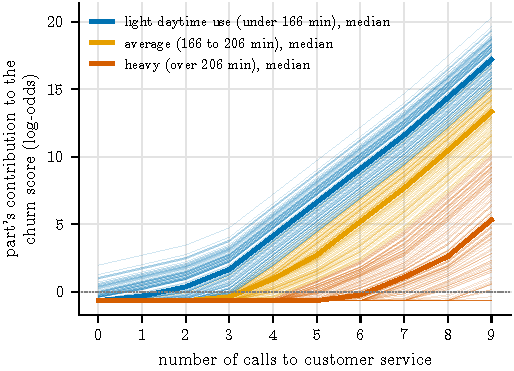
\includegraphics[width=0.7\textwidth]{figures/exp2/exp2-worked-ice}
  \caption{Churn seed 5, the part \emph{Service calls and daytime charge}: individual conditional expectation (ICE) curves of the part's contribution to the churn score as the number of customer-service calls is set from 0 to 9, for 400 training customers (every tenth), coloured by the customer's daytime minutes (thirds of the training rows), with the median curve of each third. The contribution is the change in log-odds when the part's output is replaced by its training baseline (the value the switch-off check uses), so 0 means the part adds nothing beyond its average. The part reads the daytime charge, which is a fixed rate times the daytime minutes (US\$\,0.17 per minute, exact to 0.005 on the training rows).}
  \label{fig:exp2-worked-ice}
\end{figure}
